\begin{figure}[!htbp]
    \centering
    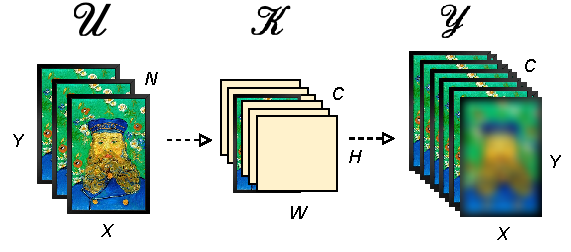
\includegraphics[width=0.45\textwidth]{\fighome/convdrawio.pdf}
    \vspace{-1.5em}
    \caption{\textbf{Depiction of a standard convolutional layer.} 
    Here $\mytensor{U} \in \R^{N\times X \times Y}$ is an $N$-stacked batch of $X\times Y$ images (Vincent van Gogh's \textit{Portrait of Joseph Roulin}). This batch is fed through a $4^\th$-order convolutional tensor $\mytensor{K}\in\R^{N \times C \times H \times W}$, where $H$ and $W$ are the kernel height and width, respectively, and $C$ is the number of output channels. (The kernel has been decomposed along its output channel mode by its matricized slices. Furthermore, we are not depicting the $N$-dimensional batch mode of each slice.) After a max-padded blurring convolution between the mode pairs $(X,H)$ and $(Y,W)$ and contraction over the $N$-dimensional batch mode, the output is a third order tensor $\mytensor{Y} \in\R^{X \times Y \times C}$.}
    \label{fig:conv-layer}
\end{figure}